\chapter{数列、数学归纳法、数列的极限}

\section{数列的定义}

\noindent
\begin{minipage}{.5\textwidth}
    \CTEXindent
我们看下面的例子:

图5.1表示堆放的钢管,
共堆放了7层,自上而下各层
的钢管数排列成一列数:
\[4,\quad 5,\quad 6,\quad 7,\quad 8,\quad 9,\quad 10\]

自然数$1,2,3,4,5,\ldots$的倒数排列成一列数:
\[1,\quad \frac{1}{2},\quad \frac{1}{3},\quad \frac{1}{4},\quad \frac{1}{5},\quad\ldots\]
\end{minipage}\hfill
\begin{minipage}{.4\textwidth}
    \centering
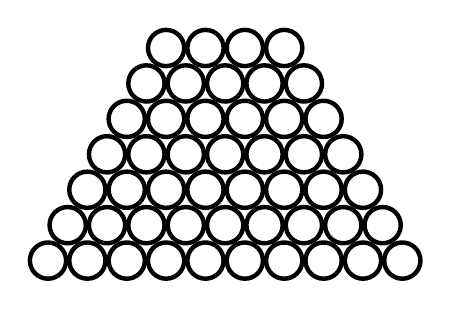
\begin{tikzpicture}
  \foreach \x in {1,2,3,...,10}
{
    \draw[ultra thick](\x/2,0)circle(.23);
}  
\foreach \x in {1,2,3,...,9}
{
    \draw[ultra thick](\x/2+.25,.45)circle(.23);
}  
\foreach \x in {1,2,3,...,8}
{
    \draw[ultra thick](\x/2+.5,.9)circle(.23);
}  
\foreach \x in {1,2,3,...,7}
{
    \draw[ultra thick](\x/2+.75,.45*3)circle(.23);
}  
\foreach \x in {1,2,3,...,6}
{
    \draw[ultra thick](\x/2+1,.9*2)circle(.23);
}  
\foreach \x in {1,2,3,...,5}
{
    \draw[ultra thick](\x/2+1.25,.45*5)circle(.23);
}  
\foreach \x in {1,2,3,4}
{
    \draw[ultra thick](\x/2+1.5,.9*3)circle(.23);
}  



\end{tikzpicture}
\captionof{figure}{ }

\end{minipage}

$\sqrt{2}$的精确到$1, 0.1, 0.01, 0.001,\ldots$的不足近似值
排列成一列数:
\[1,\quad 1.4,\quad 1.41,\quad 1.414,\quad \ldots\]    

$-1$的1次幂,2次幂,3次幂,4次幂,……排列成一列
数:
\[-1,\quad 1,\quad -1,\quad 1, \quad\ldots\]

再看下面的例子:

函数$y=\frac{1}{x^{3}}$, 当$x$依次取$1,2,3,\ldots,n\; (n\in\N)$时,得到一列数:
\[1, \frac 18, \frac {1}{27}, \ldots, \frac {1}{m^{3}}\]

函数$y=x^{2}-1$, 当$x$依次取$1,2,3,4,\ldots,n\; (n\in \N)$
时,得到一列数
$$0,\; 3,\; 8,\; 15,\ldots,\; n^{2}-1$$

象上面这些例子,按一定顺序排列的一列数叫做\textbf{数列}。数列中的每一个数都叫做这个数列的\textbf{项},各项依次叫做这个数列的第1项(或首项),第2项,第3项,……,第$n$项.

在一个数列中,它的任一项的数值,由它所对应的项数唯一确定,因此数列中各项的值是其项数的 函数,即$a_n=f(n)$, 其中$a_n$表示第$n$项。$n$为自变量$(n\in\mathbb{N})$, 第$n$项为$a_n$的数列记作$\{a_n\}$.

\section{数列的表示法}
数列实质上就是其定义域是自然数集$\N$(或$\N$的有限子
集$\{1,2,\ldots,n\}$)的函数,因此数列的表示方法与过去所学
的函数的表示方法完全类似。

\subsection{列表法表示数列}
将数列的各项依次列举出来:
\[a_1,a_2,a_3,a_4,\ldots, a_n, \ldots\]
其中$a_n$
表示数列第$n$项的数值,$n$是它的项数。显然$a_n$是$n$的函
数。

\subsection{图象法表示数列}

\begin{figure}[htp]
    \centering
\begin{tikzpicture}[>=stealth, scale=.5]
\begin{scope}
\draw[->](-1,0)--(7,0)node[below]{$n$};
\draw[->](0,-3)--(0,8)node[left]{$a_n$};
\foreach \x/\y in {3/1,4/3,5/5,6/7}
{
    \draw[dashed](0,\y)node[left]{$\y$}--(\x, \y)--(\x,0)node[below]{$\x$};
}
\foreach \x/\y in {1/-2,2/-1}
{
    \draw[dashed](0,\y)node[left]{$\y$}--(\x, \y)--(\x,0)node[above]{$\x$};
}
\node[below left]{$O$};
\node at (4,-2){(1)};
\end{scope}
\begin{scope}[xshift=12cm]
    \draw[->](-1,0)--(7,0)node[below]{$n$};
\draw[->](0,-1)--(0,7)node[left]{$a_n$};
\foreach \x in {1,2,3,4,5,6}
{
    \draw[dashed](\x,0)node[below]{$\x$}--(\x,{5-5/(\x+1)})--(0,{5-5/(\x+1)});
}
\node[below left]{$O$};
\node at (3,-2){(2)};
\node at (0,2.5)[left]{$\tfrac{1}{2}$};
\node at (0,4.16)[left]{$\tfrac{5}{6}$};
\draw(0,5)node[left]{1}--(.1,5);

\end{scope}
\end{tikzpicture}
    \caption{}
\end{figure}

图5.2(1)表示数列$-3,-1,1,3,5,7,\ldots$; 图5.2(2)表示数列
$\frac{1}{2},\frac{2}{3},\frac{3}{4},\frac{4}{5},\frac{5}{6},\ldots$.

用图象法表示数列时,图象是由直角坐标系中的一些孤
立点组成,其中每一个点$(n,a_n)$
的横坐标$n$表示项数,纵坐标$a_n$表示该项的值,用图象表示数列时,其两个坐标轴上的单位可以不同。

\subsection{解析法表示数列}
如果数列的第$n$项$a_n$能用项数$n$的解析式表示为:
$a_n=f(n)\; (n\in\N)$。这种表示方法称为解析法,这个解析式叫做数列的\textbf{通项公式}。

图5.2(1)所表示的数列的通项公式
$a_n=2n-5$; 图
5.2(2)所表示的数列的通项公式为$a_n=\frac{n}{n+1}$.

不是所有的数列都能用解析法来表示。例如$\sqrt{2}$
的精
确到$1,0.1,0.01,0.001,\ldots$的不足近似值组成的数列$1,
1.4,1.41,1.414,\ldots$就没有通项公式。

\subsection{用递推式表示数列}
有时数列可以用它的前几项的值(称初始条件或初始
值),和数列中相邻若干项间的关系式(称递推式)给出。例
如一个数列$\{a_n\}$
中,
$a_1=1$,
$a_{n+1}=2a_{n}+1\; (n\in\N)$
,这个数列
就是$1,3,7,15,31,63,\ldots$; 又如数列$2,5,8,11,14,
\ldots$, 可以表示为:
$a_1=2$, $a_{n+1}=a_n+3$.

\begin{ex}
    按照下列条件,写出数列的前五项。
\begin{enumerate}
    \item 数列的通项公式是:
\begin{multicols}{2}
\begin{enumerate}[(1)]
    \item $a_n=-3n+1$
    \item $a_n=\left(\frac{1}{2}\right)^n$
    \item $a_n=\frac{2n-1}{n+1}$
    \item $a_n=n^2+2$
\end{enumerate}    
\end{multicols}
\item 数列$\{a_n\}$中,已知
$a_1=2$,且$(n\in\N)$.
\item 数列$\{a_n\}$的图象如图5.3.
\end{enumerate}
\end{ex}

\begin{center}
\begin{tikzpicture}[>=stealth, scale=.6]
 \draw[->](-1,0)--(7,0)node[below]{$n$};
\draw[->](0,-3)--(0,4)node[right]{$a_n$};
\foreach \x in {1,2,3,4,5,6}
{
   \draw(\x,0)node[below]{$\x$}--(\x,.1);
}
\foreach \x in {1,2,3,-1,-2}
{
   \draw(0,\x)node[left]{$\x$}--(.1,\x);
}
\draw[dashed](0,-2)--(3,-2)--(3,0);
\draw[dashed](0,-1)--(5,-1)--(5,0);
\draw[dashed](0,.5)node[left]{$\tfrac{1}{2}$}--(6,.5)--(6,0);
\draw[dashed](0,3)--(2,3)--(2,0);
\draw[dashed](0,1)--(4,1)--(4,0);
\node[below left]{$O$};
\end{tikzpicture}
\captionof{figure}{ }
\end{center}

\section{简单数列的通项公式的求法}
用语言叙述或用列表法给出的一些数列的前几项,我们
可以利用归纳的办法,写出它们的通项公式。

\begin{example}
    写出下列各数列的通项公式。
\begin{enumerate}[(1)]
\item 自然数的倒数组成的数列;
\item 每项的值都比项数的立方少2的数列;
\item $-1$的自然数次幂组成的数列。
\end{enumerate}
\end{example}

\begin{solution}
\begin{multicols}{3}
  \begin{enumerate}[(1)]
    \item $a_n=\frac{1}{n}$
    \item $a_n=n^3-2$
    \item $a_n=(-1)^n$
\end{enumerate}  
\end{multicols}
\end{solution}

\begin{example}
    写出下列各数列的一个通项公式,使其前六项分
别是:
\begin{enumerate}[(1)]
\item  $\frac 12,\; \frac 34, \;\frac 78,\; \frac {15}{16} , \; \frac {31}{32} , \; \frac {63}{64}$
\item $2,\; -6,\; 18,\; -54,\; 162,\; -486$
\item $-1,\; \frac{3}{2},\; -\frac{1}{3},\; \frac{3}{4},\; -\frac{1}{5},\; \frac{3}{6}$
\item $9,\; 99,\; 999,\; 9999,\; 99999,\; 999999$
\end{enumerate}

\end{example}

\begin{solution}
\begin{enumerate}[(1)]
    \item 分母为$2^n$,分子均比分母少1, 所以数列的通
    项公式为$a_n=\frac{2^n-1}{2^n}$
    \item 分析数列的前6项发现,第1项是2, 第2项是
    2的$-3$倍,第3项又是第二项的$-3$倍,以此类推,可归纳
    出其通项公式为
    $a_n=2\x(-3)^{n-1}$
    \item 数列各项的分母依次为$1,2,\ldots$, 恰与项数相同;
    各项的分子为$1,3,1,3,\ldots$, 可以说是第1项比2少1,
    第2项比2多1, 以此类推;又数列相邻两项值的符号相
    反,且第1项为负值,因此可用符号$(-1)^n$来表示,由此归
    纳可得通项公式为
    $a_n=(-1)^{n}\frac{2+(-1)^n}{n}$.
    \item 数列第1项可改写为$10-1$, 第2项为
    $10^2-1$,……
    故通项公式为$a_n=10^n-1$.
\end{enumerate}
\end{solution}

\begin{rmk}
\begin{enumerate}[(1)]
    \item  分析数列中各项的值与项数间的关系,从而
    归纳出通项公式,是求数列通项公式的最基本的方法。
    \item 给出数列的前几项,求这个数列的通项公式时,
    其通项公式并不是唯一的。事实上,满足一个数列的前若干
    项的通项公式可以有无穷多个。例如,上例中的(1)的通
    项公式可以写成:
\[a_n=\frac{2^n-1}{2^n}+(n-1)(n-2)(n-3)(n-4)(n-5)(n-6)\cdot f(n)\]
(其中$f(n)$
是含$n$的任何一个函数式),其前六项均符合要
求,这是因为公式的后一部分,当$n$依次取$1,2,3,4,5,
6$时,其值都是0.
\end{enumerate}
\end{rmk}

\begin{ex}
\begin{enumerate}
    \item 写出数列的一个通项公式,使得数列的前五项分别是
\begin{enumerate}[(1)]
    \item $15,\; 25,\; 35,\; 45,\; 55$
    \item $1,\; -\frac{1}{2},\; \frac{1}{4},\; -\frac{1}{8},\; \frac{1}{16}$
    \item $1,\; 3,\; 5,\; 7,\; 9$
    \item $1-\frac{1}{2},\; \frac{1}{2}-\frac{1}{3},\; \frac{1}{3}-\frac{1}{4},\; \frac{1}{4}-\frac{1}{5},\; \frac{1}{5}-\frac{1}{6}$
    \item $0,\; -5,\; 8,\; -17,\; 24$
    \item $3,\; 33,\; 333,\; 3333,\; 33333$
\end{enumerate}
\item 观察下列数列的特点,用适当的数填空并对每一个数列各
写出一个通项公式:
\begin{enumerate}[(1)]
    \item $2,\; 4,\; (\quad ),\; 8,\; 10,\; (\quad ),\;14$
    \item $2,\;4,\;(\quad),\;16,\;32,\;(\quad),\;128,\;(\quad)$
    \item $(\quad),\;4,\;9,\;16,\;(\quad),\;(\quad),\;49,\;64,\;(\quad)$
    \item $(\quad),\;4,\;3,\;2,\;1,\;(\quad ),\; -1,\; (\quad ),\;(\quad )$
    \item $1,\;\sqrt{2},\;(\quad),\; 2,\;\sqrt{5},\; (\quad),\;(\quad),\; 2\sqrt{2}$
    \item $\frac{1}{6},\; \frac{1}{12},\; \frac{1}{20},\;(\quad),\;\frac{1}{42},\;(\quad),\;\frac{1}{72}$
\end{enumerate}
\item 已知数列的通项公式,试判断后面所给的数是否是数列
中的项,如果是,是第几项。
\begin{enumerate}[(1)]
    \item $a_n=n(n+2),\qquad$  (a) 142,\quad (b) 175
    \item $a_n=\frac{2n-1}{3n+2},\qquad $ (a) $\frac{3}{5}$,\quad (b) $\frac{17}{26}$
    \item $a_n=\frac{n^2+3n}{n+1},\qquad $ (a) $\frac{182}{13}$,\quad (b) $\frac{350}{13}$
\end{enumerate}
\end{enumerate}
\end{ex}

\section{数列的分类}

\subsection*{按照数列的项数,可将数列分成有穷数列和无穷数
列}

有穷数列:如果在某一项的后面不再有任何项,这个数
列叫做\textbf{有穷数列}。例如,在前一百个自然数中,一切质数组
成的数列$2,3,5,7,11,13,\ldots,97$是有穷数列。

无穷数列:如果在任何一项的后面都有跟随着的项,这
个数列叫做\textbf{无穷数列}。例如,自然数中所有奇数组成的数列,是无穷数列。

当用列表法表示数列时,写出末项的,表示有穷数列,
如$1,\frac{1}{2},\frac{1}{4},\frac{1}{8},\ldots,\frac{1}{2^{n-1}}$
表示有穷数列;写不出末
项的,则表示无穷数列,如$2,4,6,8,\ldots,2n,\ldots$表示
无穷数列。

\subsection*{按照项与项之间的大小关系,可将数列分成常数列,
递增数列,递减数列和摆动数列}

\begin{enumerate}[(1)]
\item 常数列:数列中各项的值都相等的数列叫\textbf{常数
列}。如$3,3,3,\ldots,3,\ldots$就是常数列;
\item 递增数列:一个数列从第2项起,每一项都大于
它的前面的一项,即
$a_{n+1}>a_n\; (n\in\N)$
,这样的数列叫做\textbf{递增
数列}。例如,自然数的平方组成的数列$1,4,9,16,\ldots,
n^2,\ldots$就是递增数列。
\item 递减数列:一个数列从第2项起,每一项都小于
它的前面的一项,即
$a_{n+1}<a_n\; (n\in\N)$
,这样的数列叫做\textbf{递减数列}。例如,自然数的倒数组成的数列$1,\frac{1}{2},\frac{1}{3},\frac{1}{4},\ldots,\frac{1}{n},\ldots$就是递减数列。

递增数列与递减数列,统称\textbf{单调数列}。

\item 摆动数列:一个数列,从第2项起,有些项大于
它的前一项,有些项又小于它的前一项,这样的数列叫做\textbf{摆
动数列}.例如数列$1,-2,4,-8,16,\ldots, (-2)^{n-1},\ldots$
是摆动数列。
\end{enumerate}

\begin{example}
    判断下列数列是递增数列、递减数列,还是摆动数
列?数列的通项公式如下:
\begin{multicols}{2}
\begin{enumerate}[(1)]
\item $a_n=2n+5$
\item $a_n=-3n+1$
\item $a_n=2\x\left(-\frac{1}{3}\right)^n$
\item $a_n=-\frac{1}{2}\x5^{n-1}$
\item $a_n=\frac{2n-3}{n+1}$
\end{enumerate}
\end{multicols}
\end{example}

\begin{solution}
判断数列的增减性要根据递增数列、递减数列的定
义,即计算
$a_{n+1}-a_n$
,并判断其值的正负。但对摆动数列,则
可写出数列的若干项予以判断。
\begin{enumerate}[(1)]
    \item $\because\quad a_{n+1}-a_n=[2(n+1)+5]-(2n+5)=2>0$
    
$\therefore\quad $数列$\{2n+5\}$
是递增数列。

\item $\because\quad a_{n+1}-a_n=[-3(n+1)+1]-(-3n+1)=-3<0$
    
$\therefore\quad $数列$\{-3n+1\}$
是递减数列。
\item 数列的前三项是:$-\frac{2}{3},\; \frac{2}{9},\; -\frac{2}{27}$,显然它是摆动数列。

\item \[\begin{split}
    \because\quad a_{n+1}-a_n&=-\frac{1}{2}\x 5^n-\left[-\frac{1}{2}\x 5^{n-1}\right]\\
    &=-\frac{1}{2}\x 5^{n-1}(5-1)=-2\x 5^{n-1}<0
\end{split}\]

$\therefore\quad $数列$\left\{-\frac{1}{2}\x 5^{n-1}\right\}$
为递减数列。

\item \[\begin{split}
    \because\quad a_{n+1}-a_n&=  \frac{2(n+1)-3}{(n+1)+1}-\frac{2n-3}{n+1}\\
    &=\frac{(2n^2+n-1)-(2n^2+n-6)}{(n+2)(n+1)}=\frac{5}{(n+2)(n+1)}>0
\end{split}\]

$\therefore\quad $数列$\left\{\frac{2n-3}{n+1}\right\}$
是递增数列。
\end{enumerate}
\end{solution}

\begin{rmk}
    这里数列的“增减性”的判断方法和函数
$f(x)$的增减性的判断方法类似。
\end{rmk}

\section{数列的前$n$项和}
数列$\{a_n\}$的前$n$项的和是指
$a_1+a_2+\cdots+a_n$,记作$S_n$,

$S_1$表示前一项之和,所以$S_1=a_1$;

$S_2$表示前两项之和,所以
$S_2=a_1+a_2$;

………………

$S_{n-1}$表示前$n-1$项之和,所以
$S_{n-1}=a_1+a_2+\cdots+a_{n-1}$

$S_n$表示前$n$项之和,所
以$S_n=a_1+a_2+\cdots+a_n$.

因此,只有当
$n\ge 1$时,$S_n$才是有意义的,例如$S_{n-1}$,只有当$n\ge 2$时,才有意义.

由$S_n$的含义可知,当$n\geqslant2$时,$a_n=S_n-S_{n-1}$, 而当$n=1$时,$a_1=S_1$。这就是$S_n$与$a_n$之间的关系:
$$a_n=\begin{cases}
    S_1& n=1\\
    S_n-S_{n-1} &n\geqslant2 
\end{cases}$$

\begin{example}
    已知数列的前$n$项和,求数列的通项公式。
\begin{multicols}{3}
\begin{enumerate}[(1)]
    \item $S_{n}= n^2- 2n+ 2$
    \item $S_{n}= 3^{n}- 2$
    \item $S_{n}=\frac{3^{n}-2^{n}}{2^{n}}$
\end{enumerate}    
\end{multicols}
\end{example}

\begin{solution}
\begin{enumerate}[(1)]
    \item $n= 1$时, $a_{1}= S_{1}= 1$
    
    $n\geqslant2$时,$a_{n}=S_{n}-S_{n-1}=(n^2-2n+2)-[(n-1)^2-2(n-1)+2]=2n-3$

又$n=1$时,$2n-3=-1\ne a_1$,

$\therefore\quad $通项公式为$a_n=\begin{cases}
    1,&n=1\\
    2n-3,&n\ge 2
\end{cases}$

\item $n= 1$时, $a_{1}= S_{1}= 1$
    
$n\geqslant2$时,$a_{n}=S_{n}-S_{n-1}=(3^n-2)-(3^{n-1}-2)=3^{n}-3^{n-1}=2\cdot 3^{n-1}$

又$n=1$时,$2\cdot 3^{n-1}=2\ne a_1$,

$\therefore\quad $通项公式为$a_n=\begin{cases}
1,&n=1\\
2\cdot 3^{n-1},&n\ge 2
\end{cases}$

\item $n= 1$时, $a_{1}= S_{1}= \frac{3-2}{2}=\frac{1}{2}$
    
$n\geqslant2$时,$a_{n}=S_{n}-S_{n-1}=\frac{1}{2}\cdot\left(\frac{3}{2}\right)^{n-1}$

又$n=1$时,$\frac{1}{2}\cdot\left(\frac{3}{2}\right)^{n-1}=\frac{1}{2}= a_1$,

$\therefore\quad $通项公式为$a_n=\frac{1}{2}\cdot\left(\frac{3}{2}\right)^{n-1}\quad (n\in\N)$
\end{enumerate}
\end{solution}

\begin{rmk}
\begin{enumerate}[(1)]
    \item $a_n=\begin{cases}
        S_1,&n=1\\
        S_n-S_{n-1},&n\ge 2
    \end{cases}$相当于分
    段函数的表达式。
    \item 若当由
    $ S_n-S_{n-1}\; (n\ge 2)$
    得到的$a_n$的解析式中,把
    $n=1$代入后的值恰好等于$a_1$时,要把通项公式写成统一的表
    达式,如本例中的(3).
\end{enumerate}
\end{rmk}


\begin{ex}
    已知数列$\{a_n\}$
的前$n$项的和$S_n$, 求它的通项公式:
\begin{enumerate}
    \item $S_n=a\cdot n^2+b\cdot n\quad \text{($a$、$b$为已知常数)}$
    \item   $S_{n}=a\cdot n^{2}+b\cdot n+c\quad  \text{($a$、$b$、$c$为已知常数)}$
    \item  $S_n=n^3+n-1$
    \item  $S_{n}=2\cdot 3^{n}-1$
    \item  $S_{n}=a\cdot b^{n-1}\quad (a,b\neq0)$
    \item  $S_{n}=a\cdot n$
\end{enumerate}
\end{ex}

\section*{习题一}
\begin{center}
    \bfseries A
\end{center}

\begin{enumerate}
    \item 写出下列各数列的一个通项公式,使它的前几项分别
    是:
\begin{multicols}{2}
\begin{enumerate}[(1)]
    \item $1,\; -2,\; 3,\; -4,\; 5$
    \item $0,\; 3,\; 8,\; 15,\; 24$
    \item $2,\; 7,\; 28,\; 63,\; 126$
    \item $1,\; -\frac{1}{3},\; \frac{1}{9},\; -\frac{1}{27},\; \frac{1}{81}$
    \item $\frac{1}{3},\; \frac{1}{8},\; \frac{1}{15},\; \frac{1}{24},\; \frac{1}{35}$
    \item $5,\; 55,\; 555,\; 5555$
    \item $1,\; 0,\; -1,\; 0,\; 1,\; 0,\; -1,\; 0$
    \item $2,\; 0,\; 2,\; 0,\; 2,\; 0$
\end{enumerate}    
\end{multicols}

\item 按照所给条件分别写出数列的前5项:
\begin{enumerate}[(1)]
    \item 通项公式为$a_n=\frac{(-1)^{n+1}}{n}$
    \item 通项公式为$a_n=-2^{n-1}+3$
    \item 若$a_1=1$, $a_{n+1}=1+\frac{1}{a_n}\; (n\in\N)$
    \item 若$a_1=5$, $a_{n+1}={a_n}+3\; (n\in\N)$
    \item 若$a_1=2$, $a_{n+1}=2{a_n}\; (n\in\N)$
    \item 若$a_1=3$, $a_2=9$, $a_{n+2}=a_{n+1}-{a_n}\; (n\in\N)$
    \item 若$a_1=1$, $a_{n+1}=a_n+\frac{1}{a_n}\; (n\in\N)$
    \item 若$a_1=1$, $a_{n+1}=\frac{2a_n}{a_n+2}\; (n\in\N)$
\end{enumerate}

\item 由$\{a_n\}$的前$n$项和$S_n$,求它的通项公式
\begin{multicols}{3}
\begin{enumerate}[(1)]
    \item $S_n=n^2+2n+1$
    \item $S_n=2\cdot 3^n-1$
    \item $S_n=(-1)^{n+1}\cdot n$
\end{enumerate}
\end{multicols}

\item 已知$\{a_n\}$的前$n$项和为$S_n=2n^3-3n$, 
则$a_5+a_6=\blank$; $a_8+a_9+a_{10}=\blank$.
\end{enumerate}

\begin{center}
    \bfseries B
\end{center}

\begin{enumerate}\setcounter{enumi}{4}
    \item 判断无穷数列是递增数列、递减数列,还是摆动数列?并
    给以证明。它们的通项公式分别是:
\begin{multicols}{2}
\begin{enumerate}[(1)]
    \item $a_n=3n-5$
    \item $a_n=-2n+5$
    \item $a_n=\frac{4}{n}$
    \item $a_n=\left(\frac{1}{3}\right)^{n+1}$
    \item $a_n=\lg n$
    \item $a_n=\sin\frac{n\pi}{2}$
    \item $a_n=n^3$
    \item $a_n=\frac{3n-2}{n+1}$
    \item $a_n=2-\frac{3}{n+1}$
    \item $a_n=n^2+2n-3$
    \item $a_n=a\cdot \left(\frac{1}{2}\right)^n$ (其中$a\ne 0$)
\end{enumerate}
\end{multicols}
\end{enumerate}

\section{等差数列的有关概念}


观察下面的数列:
\begin{align}
&1,\; 4,\; 7,\; 10,\; 13,\; \ldots \tag{1}\\
&5,\; 0,\; -5,\; -10,\; -15,\; \ldots \tag{2}\\
&2,\; 2,\; 2,\; 2,\; 2,\; \ldots \tag{3}
\end{align}

它们分别具有下述的特点:

(1)中,从第2项起,每一项与它的前一项的差都是3;

(2)中,从第2项起,每一项与它的前一项之差都是$-5$;

(3)中,从第2项起,每一项与它的前一项之差都是0.

它们的共同特点是:从第2项起,每一项与它的前一项
之差都等于同一个常数,通常把这个常数记作$d$, 即
\[a_n-a_{n-1}=d\quad \text{($n\ge 2$, \; $d$是常数)}\]
这类数列叫做\textbf{等差数列},常数$d$叫做等差数列的\textbf{公差}。上述三个等差数列的公差分别是$3,-5$和0, 数列(3)说明常数
数列一定是等差数列。

如果有三个数$x,A,y$组成等差数列,那么$A$叫做$x$和$y$
的\textbf{等差中项}。

如果$x,A,y$
成等差数列,由等差数列的定义可知$A-x=y-A$,所以
\[A=\frac{x+y}{2}\]

显然,任何两个数,都有唯一确定的等差中项。

容易看出,在一个无穷的等差数列中,从第2项起,每
一项都是它的前一项与后一项的等差中项;反之,在一个数
列中,如果从第2项起,每一项都是它的前一项与后一项的
等差中项,那么这个数列一定是等差数列。

\begin{example}
已知数列$\{a_n\}$的通项公式为
$a_n=3n-5$.
\begin{enumerate}[(1)]
\item 求证:数列$\{a_n\}$是等差数列,并求其公差;
\item 求出数列的首项及第100项;
\item 判断100和110是不是该数列中的项,如果是,是第
几项?
\end{enumerate}
\end{example}

\begin{solution}
\begin{enumerate}[(1)]
    \item 由于
    $a_n-a_{n-1}=3n-5-[3(n-1)-5]=3$(常数),所以数列
    $\{a_n\}$
    是等差数列,且公差是3.
\item $a_1=3\x1-5=-2$. $a_{100}=3\x100-5=295$.
\item 设
    $3n-5=100$,解之得
    $n=35$,所以100是数列的第
    35项。

    设
    $3n-5=110$,解之得
    $n=\frac{115}{3}$不是正整数,所以110不是数列$\{a_n\}$中的项。
\end{enumerate}
\end{solution}

\begin{example}
    求证:通项公式是
$a_n=an+b$($a$、$b$是常数)的数列$\{a_n\}$
是等差数列,且公差
$d=a$.
\end{example}

\begin{proof}
$\because\quad a_n-a_{n-1}=an+b-[a(n-1)+b]=a$,

$\therefore\quad \{a_n\}$是等差数列,且以
$a$为公差。
\end{proof}

例5.6说明当$a\ne 0$
,即通项公式是$n$的一次式时,该数列
必为等差数列,且其一次项系数恰好是此等差数列的公差。

显然,当$a=0$
时,数列是常数列,也是等差数列。

\section{等差数列的通项公式}
上面的例5.6告诉我们,一个数列的通项公式是$n$的一次
式时,该数列一定是等差数列,并且其一次项系数恰好是该
等差数列的公差。那么一个等差数列若公差$d\ne 0$时,其通项
公式是否也一定是$n$的一次式呢?

为此,我们做如下的探讨:

由等差数列的定义,有
\[\begin{split}
  a_2&=a_1+d,\\
a_3&=a_2+d=(a_1+d)+d=a_1+2d,\\
a_4&=a_3+d=(a_1+2d)+d=a_1+3d,\\
\cdots &\cdots \cdots
\end{split}\]

这样,可以归纳得出
\[a_n=a_1+(n-1)d\]
这是由对事物的部分对象的考察,观察其规律,得出的
结论。这个方法就是不完全归纳法。所得结论的正确性,今
后我们可以用数学归纳法给予证明。

这个公式,还可以用下面的方法得到

由等差数列的定义,可知
\[\begin{split}
    a_2-a_1&=d\\
    a_3-a_2&=d\\
    a_4-a_3&=d\\
    \cdots&\cdots\cdots\\
    a_{n-1}-a_{n-2}&=d\\
    a_n-a_{n-1}&=d\\
\end{split}\]

将这$n-1$个式子的等号两边分别相加,得$a_n-a_1=(n-1)d$,
即
\[a_n=a_1+(n-1)d\]
这个方法,通常称为\textbf{迭加法}。

$a_n=a_1+(n-1)d$就是用首项
$a_1$和公差$d$表示的等差数
列的\textbf{通项公式}。

$\because\quad a_n=a_1+(n-1)d=dn+(a_1-d)$

$\therefore\quad$当$d\ne 0$时,$a_n$是$n$的一次式,且一次项的系数是公差$d$.

显然,如果
$a_n=dn+(a_1-d)$
中的
$d=0$,$\{a_n\}$
也是等差数列。

结合5.6中的例5.6, 我们可以得到下述定理:

\begin{thm}
{定理1} 数列$\{a_n\}$是等差数列的充分必要条件是
$a_n=dn+b$, 其中$d$为公差,$b$为常数。
\end{thm}

用图象法表示等差数列时,点$(n,a_n)$
一定在斜率为$d$的
一条直线上。

5.6中的数列(1)可用图5.4来表示,其中点$(1,1)$,
$(2,4)$, $(3,7)$, $(4,10)$, ……都在直线
$y=3x-2$上。其中直线的斜率3, 恰好是该数列的公差。

\begin{figure}[htp]
    \centering
\begin{tikzpicture}[>=stealth, yscale=.5]
\draw[->](-1,0)--(4,0)node[right]{$n$};
\draw[->](0,-1)--(0,9)node[right]{$a_n$};
\node[below left]{$O$};
\foreach \x in {1,2,3}
{
    \draw(\x,0)node[below]{\x}--(\x,.1);
}
\foreach \x in{2,4,6,8}
{
    \draw(0,\x)node[left]{\x}--(.1,\x);
}

\draw[domain=.25:3.5, smooth, dashed]plot(\x, 3*\x-2);
\tkzDefPoints{1/1/A, 2/4/B, 3/7/C}
\tkzDrawPoints(A,B,C)
\node at (A)[right]{$(1,1)$};
\node at (B)[right]{$(2,4)$};
\node at (C)[right]{$(3,7)$};

\end{tikzpicture}
    \caption{}
\end{figure}


与确定函数式$y=kx+b$一样,要确定一个等差数列的通
项公式,需要知道两个独立条
件,例如数列中的某一项和公差,或数列中的任何两项,等等。

\begin{example}
   已知等差数列的公差为$d$, 第$m$项是
$a_m$,试求其第$n$项$a_n$. 
\end{example}

\begin{solution}
    由等差数列的通项公式可知
$a_n=a_1+(n-1)d$, 
即
\[a_m=a_1+(m-1)d\]

两式相减,得
$a_n-a_m=(n-m)d$,
即
\[a_n=a_m+(n-m)d\]
\end{solution}

此例说明:等差数列的通项公式,可以用数列中的任何
一项及公差来表示。特别当$m=1$时,就是
\[a_n=a_1+(n-1)d\]

\begin{example}
    等差数列的第5项是20,公差是3,求它的第50
项。
\end{example}

\begin{solution}
 \textbf{解法一:} $\because\quad a_5=a_1+4d$,

$\therefore\quad a_1+4\x3=20$,解得$a_1=8$

$\therefore\quad a_{50}=a_1+49d=8+49\x3=155$.

\textbf{解法二:} 因为
$d=3$,由定理1可设数列的通项公式为
\[a_n=3n+b\]
$\therefore\quad a_5=3\x5+b=20$

$\therefore\quad b=5$,于是
\[a_{50}=3\x50+5=155\]

\textbf{解法三:} 由例5.7的结论,有
\[a_{50}=a_5+(50-5)d\]
于是
\[a_{50}=20+45\x3=155\]
\end{solution}

\begin{example}
    梯子共有12级,从上面数第四级的宽是54cm, 最
低一级宽110cm, 已知各级的宽度成等差数列,试计算梯子
各级的宽。
\end{example}

\begin{solution}
    用$\{a_n\}$表示题中的等差数列,其公差为
$d$, 设$a_n=dn+b$,由已知
$a_4=54$,$a_{12}=110$,所以
\[\begin{cases}
    54=d\cdot 4+b\\
    110=d\cdot 12+b
\end{cases}\]
解关于$d$、$b$的方程组,得$d=7$,$b=26$
,于是
\[a_n=7n+26\]
\[\begin{split}
\therefore\quad a_1&=7\x 1+26=33\\
a_2&=7\x2+26=40\\
a_3&=7\x3+26=47\\
\cdots & \cdots\cdots
\end{split}\]

答:梯子自上而下各级的宽度依次为33, 40, 47, 54, 
61, 68, 75, 82, 89, 96, 103和110(cm).
\end{solution}

\begin{example}
    在$-1$和9之间插入三个数,使这五个数组成等差
数列,求插入的三个数。
\end{example}

\begin{solution}
    设数列为$\{a_n\}$,由题意知
$a_1=-1$,$a_5=9$。

由等差数列通项公式,有
\[d=\frac{a_n-a_1}{n-1}=\frac{9-(-1)}{5-1}=2.5\]

$\therefore\quad a_2=1.5,\quad a_3=4,\quad a_4=6.5$

答:插入的三个数分别为1.5, 4和6.5.

\textbf{另解:}因为等差数列$\{a_n\}$
共有5项,所以$a_3$是$a_1$和$a_5$的
等差中项,即
\[a_3=\frac{-1+9}{2}=4\]

又$a_2$是$a_1$和$a_3$的等差中项,
$a_4$是$a_3$和$a_5$的等差中项,故
\[a_3=\frac{-1+4}{2}=1.5,\quad a_4=\frac{4+9}{2}=6.5\]

答:插入的三个数分别为1.5, 4和6.5.
\end{solution}

\begin{example}
已知$a^2,\;b^2,\;c^2$成等差数列,且$b+c,\;c+a,\;a+b$均不为零,

求证:$\frac{1}{b+c},\;\frac{1}{c+a},\; \frac{1}{a+b}$也成等差数列.
\end{example}

\begin{solution}
因为$a^2,b^2,c^2$成等差数列,所以
$2b^2=a^2+c^2$,于是
\[\begin{split}
\frac{1}{b+c}+\frac{1}{a+b}&=\frac{a+b+b+c}{ab+b^2+ac+bc}=\frac{a+2b+c}{ab+\frac{a^2+c^2}{2}+ac+bc}\\
&=\frac{2(a+2b+c)}{2ab+a^2+c^2+2ac+2bc}\\
&=\frac{2(a+2b+c)}{(a+c)(a+c+2b)}=\frac{2}{a+c}
\end{split}\]

$\therefore\quad \frac{1}{b+c},\;\frac{1}{c+a},\; \frac{1}{a+b}$也成等差数列.
\end{solution}



\begin{example}
    已知一个直角形的三条边成等差数列,求证它们的
比是3:4:5.
\end{example}


\begin{solution}
    将成等差数列的三边的长从小到大排列,它们可以
表示为
$a-d$, $a$, $a+d$,
其中
$a-d>0$, $d>0$, $d$
就是它们的
公差。由于它们是直角三角形的三边的长,根据勾股定理,得
到
\[(a-d)^2+a^2=(a+d)^2\]
解之得$a=4d$, 
从而,三角形三边长依次为$3d$, $4d$和$5d$,
因此,三条边之比为$3:4:5$.
\end{solution}

\begin{rmk}
此例中设成等差数列的三数为$x-d$
,$x$和$x+d$($d$为公差)。可简化运算过程。若四数成等差数列时,可设为
$x-3d$, $x-d$, $x+d$和$x+3d$
,这样可用两个量$x,d$表示四
个数。但需注意这里$d$并非其公差,公差是$2d$.
\end{rmk}

\begin{example}
    设等差数列$\{a_n\}$
的公差为$d$, 求证:
\begin{enumerate}[(1)]
\item 当$d>0$时,数列是递增数列;
\item 当$d<0$时,数列是递减数列。
\end{enumerate}
\end{example}

\begin{solution}
因为$\{an\}$是等差数列,当
$d\ne 0$时它的通项公式是
$n$的一次式,且其一次项系数恰是数列的公差$d$, 即
$a_n=dn+c$.

由一次函数的性质可知:
\begin{itemize}
    \item 当$d>0$时,函数
$y=dx+c$
是增函数,故数列
$\{d_n+c\}$也为递增数列,
\item 当$d<0$时,函数
$y=dx+c$是减函数,故数列
$\{dn+c\}$
为递减数列。
\end{itemize}
\end{solution}


\begin{example}
    一个等差数列的首项是50, 公差是$-0.6$, 从第几
项开始是负数。
\end{example}

\begin{solution}    
该数列的通项公式是
$a_n=50-(n-1)\x0.6$,令
$50-(n-1)\x0.6=0$,
解之得:$$n=84.3$$

由于数列是首项为正的递减数列,所以从第85项开始是
负数。
\end{solution}





\begin{example}
设$\{a_n\}$是等差数列,$k,\ell,m,n\in\N$,若
$k+\ell=m+n$,则
$a_k+a_{\ell}=a_m+a_n$
\end{example}

\begin{proof}
    设数列的公差为$d$, 则有
\[\begin{split}
     a_k&=a_1+(k-1)d,\\
a_{\ell}&=a_1+(\ell-1)d.
\end{split}\]

$\therefore\quad a_k+a_{\ell}=2a_1+(k+\ell-2)d$

$\because\quad a_m=a_{\ell}+(m-\ell)d,\quad a_n=a_1+(n-1)d$

$\therefore\quad a_m+a_n=2a_1+(m+n-2)d$

$\because\quad k+\ell=m+n$

$\therefore\quad a_k+a_{\ell}=a_m+a_n$
\end{proof}

\begin{rmk}
    此例说明,在等差数列中,项数之和相等时,对
应的两项之和也相等,例如等差数列$\{a_n\}$
中,有
$a_5+a_{13}=a_2+a_{16}=a_8+a_{10}=\cdots$,这是等差数列的一个重要性质。

特别地
$a_1+a_n=a_2+a_{n-1}=a_3+a_{n-2}=\cdots$.
\end{rmk}

\begin{ex}
\begin{enumerate}
    \item 解下列各题:
\begin{enumerate}[(1)]
\item 求等差数列$3,\; 7,\; 11,\; \ldots$的第4,7,10项;
\item 求等差数列$10,\; 8,\; 6,\; \ldots$的第20项;
\item 求等差数列$2,\; 9,\; 16,\; \cdots$的第$n$项;
\item 求等差数列$0,\; -3\frac{1}{2},\; -7,\; \cdots$的第$n+1$项。
\end{enumerate}

\item 设等差数列$\{a_n\}$的公差为$d$, 求证:
\begin{enumerate}[(1)]
\item $d= \frac {a_{n}- a_{1}}{n- 1},\quad \left ( n\neq 1\right ) $     
\item $d= \frac {a_{n}- a_{m}}{n- m},\quad ( m\neq n) $
\end{enumerate}

\item 设$\{a_n\}$为等差数列,公差为$d$.
\begin{enumerate}[(1)]
\item 已知 $d=-\frac{1}{3}$, $a_{7}=8$, 求$a_1$;
\item 已知$a_{1}=12$, $a_{6}=27$, 求$d$;
\item  已知$a_1=3$, $a_n=21$, $d=2$, 求$n$; 
\item 已知$a_4=10$, $a_7=19$, 求$a_1$和$d$;
\item 已知$a_1=1.7$, $d=0.3$, 求证46.7是该数列中的项,并说明是第几项。
\end{enumerate}
\item 求证等差数列$\{a_n\}$中所有的奇数项组成的数列也是等 差数列,并求这个数列的公差。
\item 求下列各题中两个数的等差中项:
\begin{multicols}{2}
\begin{enumerate}[(1)]
    \item 647与895
    \item $-180$与360
    \item $\frac{\sqrt{3}+\sqrt{2}}{\sqrt{3}-\sqrt{2}}$与$\frac{\sqrt{3}-\sqrt{2}}{\sqrt{3}+\sqrt{2}}$
    \item $(a+b)^2$与$(a-b)^2$
\end{enumerate}    
\end{multicols}
\end{enumerate}
\end{ex}

\section{等差数列前$n$项的和}
我们观察下面的例子:

图5.5(1)表示有规则堆放着的钢管。

\begin{figure}[htp]
    \centering
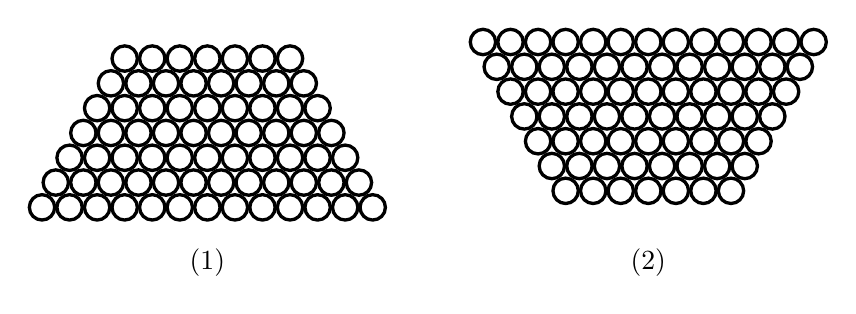
\begin{tikzpicture}[scale=.7]
\begin{scope}
 \foreach \x in {1,2,3,...,13}
{
    \draw[very thick](\x/2,0)circle(.23);
}  
\foreach \x in {1,2,3,...,12}
{
    \draw[very thick](\x/2+.25,.45)circle(.23);
}  
\foreach \x in {1,2,3,...,11}
{
    \draw[very thick](\x/2+.5,.9)circle(.23);
}  
\foreach \x in {1,2,3,...,10}
{
    \draw[very thick](\x/2+.75,.45*3)circle(.23);
}  
\foreach \x in {1,2,3,...,9}
{
    \draw[very thick](\x/2+1,.9*2)circle(.23);
}  
\foreach \x in {1,2,3,...,8}
{
    \draw[very thick](\x/2+1.25,.45*5)circle(.23);
}  
\foreach \x in {1,2,3,...,7}
{
    \draw[very thick](\x/2+1.5,.9*3)circle(.23);
}  
\node at (3.5,-1){(1)};
\end{scope}

\begin{scope}[xshift=8cm]    
\node at (3.5,-1){(2)};

 \foreach \x in {1,2,3,...,13}
{
    \draw[very thick](\x/2,-0+3)circle(.23);
}  
\foreach \x in {1,2,3,...,12}
{
    \draw[very thick](\x/2+.25,-.45+3)circle(.23);
}  
\foreach \x in {1,2,3,...,11}
{
    \draw[very thick](\x/2+.5,3-.9)circle(.23);
}  
\foreach \x in {1,2,3,...,10}
{
    \draw[very thick](\x/2+.75,3-.45*3)circle(.23);
}  
\foreach \x in {1,2,3,...,9}
{
    \draw[very thick](\x/2+1,3-.9*2)circle(.23);
}  
\foreach \x in {1,2,3,...,8}
{
    \draw[very thick](\x/2+1.25,3-.45*5)circle(.23);
}  
\foreach \x in {1,2,3,...,7}
{
    \draw[very thick](\x/2+1.5,3-.9*3)circle(.23);
}  

\end{scope}
\end{tikzpicture}
    \caption{}
\end{figure}


显然,自上而下各层的钢管数排成一个等差数列:7,8、
9、10、11、12、13.

为了求出钢管的总数,我们可以设想如图5.5(2)那样,
在这堆钢管旁边倒放着同样的一堆钢管,把两堆合起来,每
层钢管数都相等,即
\[7+13=8+12=\cdots=13+7\]

由于共有七层,因此两堆钢管总数就是:$(7+13)\x7$,
那么,所求钢管总数是
$$\frac{7+13}{2}\x7=70$$
    
一般地,设有等差数列$a_1,a_2,a_3,\ldots,a_n,\ldots$,
它的前$n$项的和记作$S_n$, 即
\[S_n=a_1+a_2+\cdots+a_n\]
根据等差数列的通项公式,上式可以写成
\[S_n=a_1+(a_1+d)+(a_1+2d)+\cdots+[a_n+(n-1)d]\]

再把项的次序反过来,$S_n$又可以写成
\[S_n=a_n+(a_n-d)+(a_n-2d)+\cdots+[a_n-(n-1)d]\]

将这两个式子相加,得
\[\begin{split}
    2S_n&=\overbrace{(a_1+a_n)+(a_1+a_n)+\cdots +(a_1+a_n)}^{n\text{个}} \\
    &=n(a_1+a_n)
\end{split}\]
由此得到等差数列$\{a_n\}$的\textbf{前$n$项的和的公式}
\begin{equation}
    S_n=\frac{n(a_1+a_n)}{2}\tag{1}
\end{equation}

若将$a_n=a_1+(n-1)d$
代入(1)式,又可得出
\begin{equation}
    S_n=na_1+\frac{n(n-1)}{2}d \tag{2}
\end{equation}

从上述求$S_n$的分析过程可见,在一个等差数列的前$n$项
中,与两端(即$a_1$和$a_n$)“等距离”的两项之和都等于首末两
项之和$a_1+a_n$。这是等差数列所具有的一个重要性质。

公式(1)和公式(2)中,分别含有四个量:$a_1,\; a_n,\;  n,\; S_n$和$a_n,\; d,\; S_n,\; n$。如果已知其中三个量,那么每个公式都可看作以其第四个量为未知数的方程,从而第四个量都可
以求出。

如果再加上前一节学的等差数列的通项公 式$a_n=a_1+$ $(n-1)d$,那么在等差数列中,常涉及到以下五个量:$a_1,\; d,\; n,\; a_n$和$S_n$, 并且它们由一组公式:通项公式 和 前$n$项和公式联系着,因此若已知其中的任何三个量,即可得到以其余两个量为未知数的方程组,从而可以求出其余的两个量。


\begin{example}
    求自然数集合中,前100个自然数的和。
\end{example}

\begin{solution}
前100个自然数,组成首项是1,公差是 1 的等差数
列,共有100项,且第100项是100,所以
$$S_{100}=\frac{1+100}2\times100=5050$$

(这正是著名的德国数学家高斯(1777—1855)在他10
岁时,很快地算出$1+2+\cdots+100$的结果时所用的解法)。 
\end{solution}









\begin{example}
图5.6表示一个堆放
铅笔的V形架,它的最下面一
层放一支铅笔,在上每一层都
比它下面一层多放一支,最上
面一层放120支,问这个V形架
上共放着多少支铅笔?

答案是7260支铅笔,请读者完成计算过程。
\end{example}

\begin{example}
    正偶数组成的数列$2,4,6,\ldots$的前多少项的和等于9900?
\end{example}

\begin{analyze}
    
\end{analyze}

















































































































